\section{Introduction}

This is the first mandatory assignment for the course SIGB F2013. In
this assignment we'll implement a simple software eye tracker. This will
be done in the programming language python with help from the opencv and
numpy libraries.

This report is an attempt to document what has been done to make this
eye tracker.

The basic structure for each section will be a short introduction of the
goal of the section, followed by the theory behind our approach ending
with a description of our actual implementation with visual aids used
for documentation. Additionally we will accompany the report with
captured videos demonstrating the usage of the eye tracker

\begin{figure}[htbp]
\centering
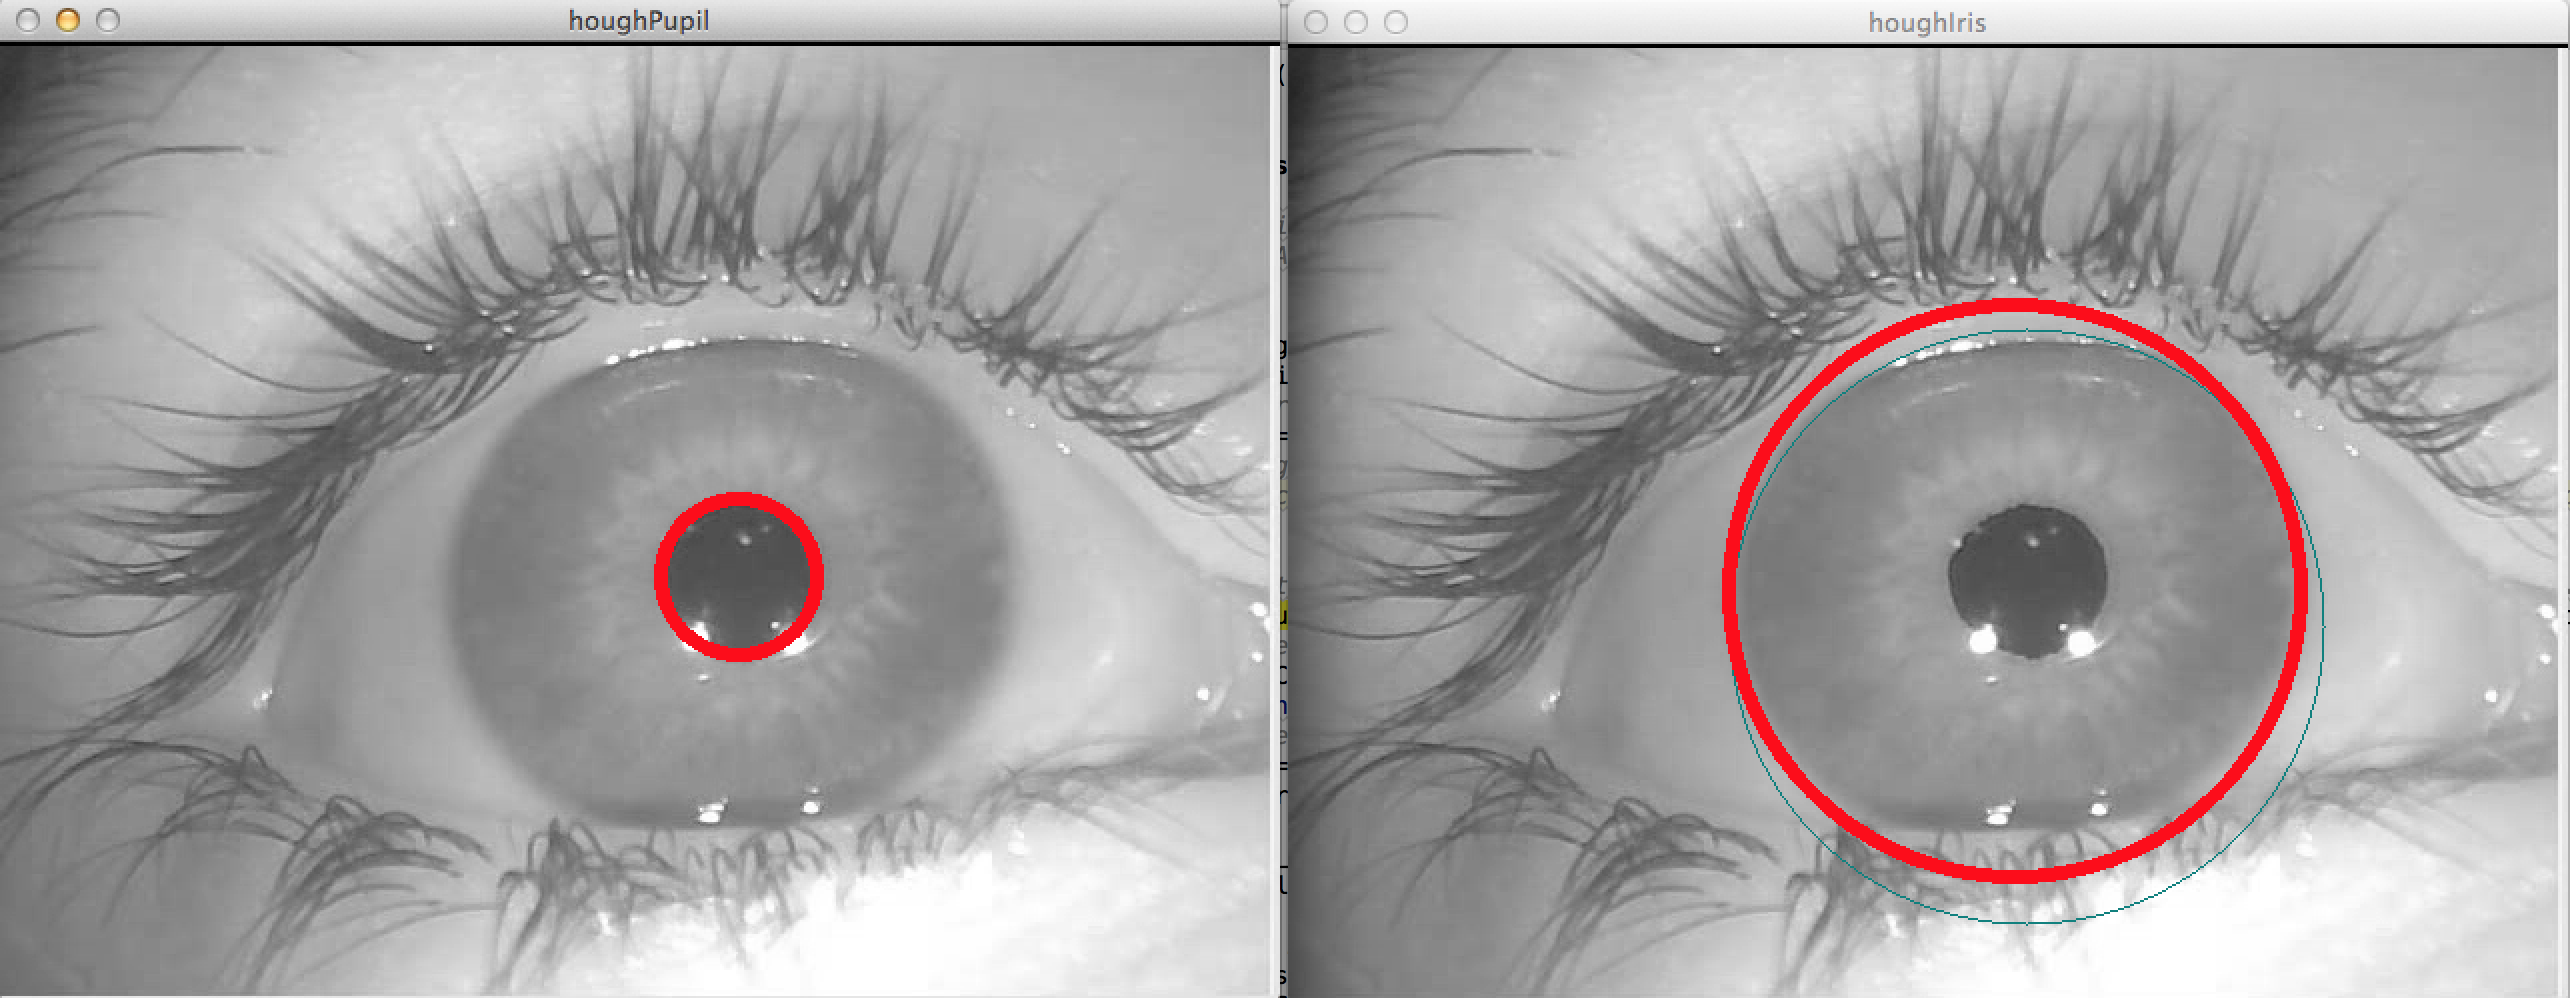
\includegraphics{pics/houghtransform.png}
\caption{Eye located with hough}
\end{figure}

\section{Pupil detection}

\subsection{Overall rationale and theory}

\subsection{Theory behind thresholding}

\subsection{Theory behind Clustering}

\subsection{K-means}

